\scanpage{14}
Soient $X$ un schéma $\mathcal A_*$-formel, et $Y$ un sous-schéma formel (lisse) de $X$. \deleted{On dit} On dit que $Y$ est un \deleted{sous} $\mathcal A_*$-schéma $\mathcal A_*$-formel s'il existe sur $Y$ une $\mathcal A_*$ structure telle que l'inclusion can. soit un $\mathcal A_*$-morphisme. Cette $\mathcal A_*$-structure est alors unique. En effet, il est immédiat qu'on peut (sans hyp. sur $Y$) trouver un \inserted{$\mathcal A_*$} morphisme $X\to Y'$ ($Y'$ un schéma $\mathcal A_*$-formel) tel que le morphisme induit $Y\to Y'$ soit un isomorphisme formel. \deleted{\unsure{Considérons}} \inserted{Considérons} l'isomorphisme inverse, et le composé
\diagram{\begin{tikzcd}[column sep=small,row sep=tiny]&Y\arrow[dr]&\\Y'\arrow[ur,"\sim"]\arrow[rr]&&X\end{tikzcd}}
Utilisant (e), on \deleted{\unsure{voit}} voit que \deleted{alors} $Y$ est un sous schéma $\mathcal A_*$-formel ssi $Y'\mathbin{-}X$ est un $\mathcal A_*$-morphisme, et alors la $\mathcal A_*$-structure de $Y$ est celle déduite.

\uline{Exemple.} La diagonale de $X\times X$ est un sous $\mathcal A_*$-schéma formel. Plus gén. celle de $X\times_Y X$ si $X\mathbin{-}Y$ est un $\mathcal A_*$ morphisme submersif. \deleted{(i.e. \unsure{grad. tang.})}
\margin{Un morphisme formel $X\to Y$ entre sch. $\mathcal A_*$-formels est un $\mathcal A_*$-morphisme ssi son graphe dans $X\times Y$ est un sous-schéma $\mathcal A_*$-formel.}
\figure{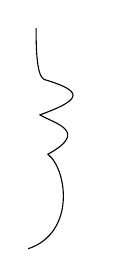
\begin{tikzpicture}\draw (0,0)..controls(.6,.2)and(.5,1)..(.25,1.2)..controls(.8,1.5)and(.3,1.6)..(.15,1.7)..controls(.7,1.9)and(.7,2)..(.2,2.15)..controls(.1,2.2)and(.1,2.6)..(.1,2.8);\end{tikzpicture}}

Soit $\mathfrak X$ un schéma sur $\mathcal O_{\mathcal A_*}(X)$ ($X$ un $\mathcal A_*$-schéma formel) muni d'une section \inserted{$s_0$} sur $\mathcal O_{\mathcal A_*}(X)$, supposons que $\mathfrak X$ soit lisse sur $\operatorname{Spec}\mathcal O_{\mathcal A_*}(X)$ aux points de cette section. Considérons le complété formel \inserted{$\hat{\mathfrak X}$} de $\mathfrak X\otimes_{\mathcal O_{\mathcal A_*}(X)}\mathcal O(X)$ le long de la section $s$ déduite de $s_0$. Alors une constr. utilisant e) permet d'y mettre une \inserted{$\mathcal A_*$-} structure, \inserted{telle que $X\to\hat{\mathfrak X}\mathbin{-}X$ soient des $\mathcal A_*$-morphismes.} (\deleted{\unsure{Ce}} $\hat{\mathfrak X}$ est défini $\mathcal A_*$-fonctoriellement dans le triple $(X,\mathfrak X,s_0)$, ce foncteur est compatible avec les images inverses par $X'\mathbin{-}X\ldots$)
\mspage{13}
